\chapter{Modelo del Negocio}	
\label{cap:reqSist}

	En este capítulo se modela la {\em Arquitectura del negocio} la cual está conformada por la Ontología del negocio ({\em Términos} y {\em Hechos del negocio}), Arquitectura de procesos y las {\em Reglas del negocio}. Primero se especifica brevemente el {\em Contexto} en el que los términos tienen significado.
	
	En las secciones \ref{sec:terminosDeNegocio} y \ref{sec:hechosDeNegocio} se presentan los Términos del negocio a manera de Glosario y por último se presentan los Hechos del negocio a manera de relaciones entre términos del negocio.

%----------------------------------------------------------
\section{Contexto}

	\cdtInstrucciones{El contexto debe explicar bajo que ambiente los términos del negocio son aplicables y proporcionar información general para su comprensión inicial.\\}
	
	
%---------------------------------------------------------
\section{Términos del Negocio}
\label{sec:terminosDeNegocio}

\begin{description}
	% Ejemplo de un término literal.
	 \item[\hypertarget{tUnidadAcademica}{Unidad académica:}] Se refiere a la institución educativa en donde los usuarios se desenvuelven diariamente.
	
	\item[\hypertarget{tUnidadAprendizaje}{Unidad de aprendizaje:}] Son los elementos que componen un plan de estudios de alguna de las carreras ofertadas en la \hyperlink{tUnidadAcademica}{unidad académica}. Es necesario que los alumnos acrediten todas sus materias para continuar con su formación académica.
	
	\item[\hypertarget{tETS}{Exámen a Título de Suficiencia (ETS):}] Prueba final que permite a los alumnos acreditar una materia reprobada, y para la cual se requiere verificación de identidad.
	
	\item[\hypertarget{tAlumno}{Alumno:}] (es un tipo de Usuario) Se refiere a las personas inscritas dentro de algún plan de estudios ofertado en la \hyperlink{tUnidadAcademica}{unidad académica}.
	
	\item[\hypertarget{tDocenteAplicador}{Docente aplicador:}] (es un tipo de Usuario) Se refiere a las personas registradas como trabajadores que dan clases a los alumnos y supervisan los ETS asignados.
	
	\item[\hypertarget{tPersonalSeguridad}{Personal de seguridad:}] (es un tipo de Usuario) Se refiere a las personas registradas como trabajadores y que permiten o no el acceso a la \hyperlink{tUnidadAcademica}{unidad académica}.
	
	\item[\hypertarget{tCodigoQR}{Código QR:}] Código único generado por el sistema que permite resolver tareas de control de acceso a las instalaciones y a servicios de autenticación.
	
	\item[\hypertarget{tSistemaVerificacion}{Sistema de verificación de la identidad:}] Conjunto de procesos que permiten validar la identidad de los alumnos que buscan aplicar un ETS.
	
	\item[\hypertarget{tCredencialEscolar}{Credencial escolar:}] Documento con datos de identificación que pueden usarse junto a los registros de inscripción a ETS para permitir o no el acceso a la \hyperlink{tUnidadAcademica}{unidad académica}.
	
	\item[\hypertarget{tControlAcceso}{Control de acceso:}] Sistema implementado para verificar y autorizar el acceso a la \hyperlink{tUnidadAcademica}{unidad académica}.
	
	\item[\hypertarget{tRegistroAcceso}{Registro de acceso:}] Historial digital que documenta los accesos permitidos y denegados, incluyendo datos de cada intento de entrada para consulta posterior.
	
%	\brTermSensor{tVelocimetro}{Velocímetro:}{Velocidad de un Vehículo.}{Kilometros/hora.}{Constantemente siempre que el \cdtRef{tVehiculo}{vehículo} esté encendido.}
\end{description}
%---------------------------------------------------------


\section{Modelo del dominio del problema}
\label{sec:terminosDeNegocio}


\subsection{Modelo del dominio del problema}

El modelo del dominio del problema se muestra en la figura~\ref{fig:modeloDeDominio}, a continuación se describen cada una de las entidades y sus relaciones.

\newpage

\begin{figure}[htbp!]
	\begin{center}
		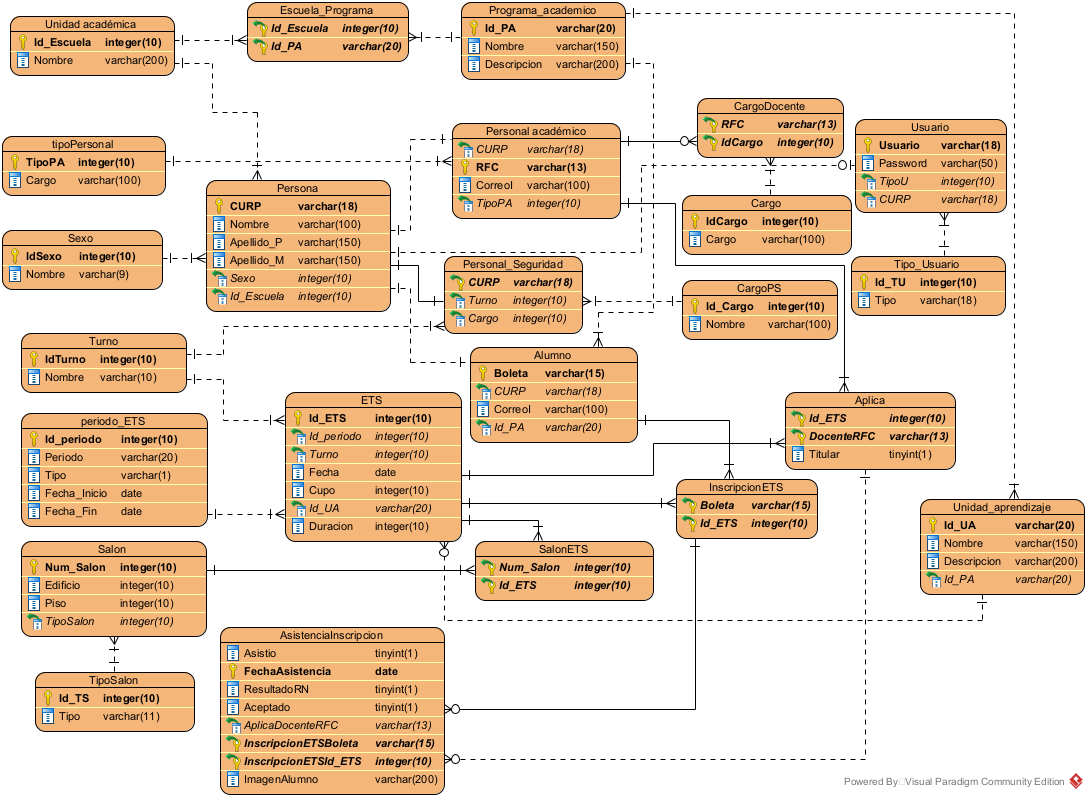
\includegraphics[angle=90,width=.85\textwidth]{images/DER}
		\caption{Modelo del dominio del problema}
		\label{fig:modeloDeDominio}
	\end{center}
\end{figure}

\newpage
%---------------------------------------------------------
\begin{cdtEntidad}{Unidad academica}{Unidad academica}
	\brAttr{Id\_escuela}{Id\_escuela}{Id}{Número de registro usado para identificar a la escuela.}{Sí}
	\brAttr{nombre}{Nombre}{Palabra}
	{Nombre de la escuela}{Sí}
%	\brAttr{ubicacion}{Ubicación}{Frase}
%	{Ubicación en la que se encuentra la escuela.}{Sí}
%	\brAttr{telefono}{Teléfono}{Teléfono}
%	{Teléfono para contactar a la escuela.}{Si}
%- - - - - - - - - - - - - - - - - - - - - - - - - - - - - 
	% \brRelComposition \brRelAgregation
%	\cdtEntityRelSection
%	\brRel{}{Programa\_académico}{ \hyperlink{Unidad academica}{Unidad académica} está compuesto por un \hyperlink{PA}{Programa académico}}	
%	\brRel{}{Persona}{Una \hyperlink{Persona}{Persona} pertenece a \hyperlink{Unidad academica}{Unidad academica}}	
\end{cdtEntidad}
%---------------------------------------------------------
\begin{cdtEntidad}{EscuelaPrograma}{Escuela\_Programa}
	\brAttr{Id\_Escuela}{Id\_Escuela}{Id}{Número de registro usado para identificar a la escuela.}{Sí}
	\brAttr{Id\_PA}{Id\_PA}{Id}
	{Identificación del programa académico que imparte la Unidad académica.}{Sí}
\end{cdtEntidad}
%---------------------------------------------------------
\begin{cdtEntidad}{PA}{Programa\_academico}
	\brAttr{Id\_PA}{Id\_PA}{Id}{Número de registro usado para identificar al programa académico.}{Sí}
	\brAttr{nombre}{Nombre}{Palabra}
	{Nombre del programa académico}{Sí}
	\brAttr{descripcion}{Descripción}{Frase}
	{Descripción que habla sobre el programa académico.}{Sí}
%- - - - - - - - - - - - - - - - - - - - - - - - - - - - -
%	\cdtEntityRelSection
%	\brRel{}{Unidad\_aprendizaje}{Un \hyperlink{PA}{Programa academico} está compuesto por una \hyperlink{UA}{Unidad de aprendizaje}}	
%	\brRel{}{Unidad academica}{Una \hyperlink{Unidad academica}{Unidad academica} está compuesta por un \hyperlink{PA}{Programa académico}}	
\end{cdtEntidad}
%---------------------------------------------------------
\begin{cdtEntidad}{Persona}{Persona}
	\brAttr{CURP}{CURP}{Id}{Código usado para identificar a las personas.}{Sí}
	\brAttr{nombre}{Nombre}{Frase corta}
	{Nombre(s) de la persona.}{Sí}
	\brAttr{ApellidoP}{Apellido\_P}{Frase corta}
	{Apellido paterno de la persona.}{Sí}
	\brAttr{ApellidoM}{Apellido\_M}{Frase corta}
	{Apellido materno de la persona.}{Sí}
	\brAttr{sexo}{Sexo}{Caracter}
	{Letra que servirá para identificar el sexo de un alumno ('M' para masculino, 'F' para femenino).}{Sí}
	\brAttr{Id\_escuela}{Id\_escuela}{Id}
	{Id de la escuela a la que pertenece la persona.}{Si}
	%- - - - - - - - - - - - - - - - - - - - - - - - - - - - -
%	\cdtEntityRelSection
%	\brRel{}{Unidad academica}{Una \hyperlink{Persona}{Persona} pertenece a una \hyperlink{Unidad academica}{Unidad academica}}	
%	\brRel{}{Docente}{Una \hyperlink{Persona}{Persona} es un \hyperlink{Docente}{Docente}}	
%	\brRel{}{Personal\_Seguridad}{Una \hyperlink{Persona}{Persona} es un \hyperlink{PS}{Personal de seguridad}}
%	\brRel{}{Alumno}{Una \hyperlink{Persona}{Persona} es un  \hyperlink{Alumno}{Alumno}}
%	\brRel{}{Usuario}{Una \hyperlink{Persona}{Persona} cuenta con un \hyperlink{Usuario}{Usuario}}
\end{cdtEntidad}
%---------------------------------------------------------
\begin{cdtEntidad}{PersonalAcademico}{Personal académico}
	\brAttr{CURP}{CURP}{Id}{Código usado para identificar a las personas.}{Sí}
	\brAttr{RFC}{RFC}{Id}
	{RFC que identifica al personal académico.}{Sí}
	\brAttr{CorreoI}{CorreoI}{Correo}
	{Correo institucional del personal académico.}{Sí}
	\brAttr{TipoPA}{TipoPA}{Id}{Número que identifica que tipo de personal académico es, ya sea, por ejemplo, un docente o personal de gestión escolar.}{Sí}
	%- - - - - - - - - - - - - - - - - - - - - - - - - - - - -
%	\cdtEntityRelSection
%	\brRel{}{CargoDocente}{Un \hyperlink{PersonalAcademico}{personal académico} puede ser un \hyperlink{CargoDocente}{Docente}}
%	\brRel{}{ETS}{Un \hyperlink{PersonalAcademico}{Docente} \hyperlink{Aplica}{Aplica} un \hyperlink{ETS}{ETS}}
%	\brRel{}{Persona}{Un \hyperlink{PersonalAcademico}{personal académico} es una \hyperlink{Persona}{Persona}}
%	\brRel{}{tipoPersonal}{Un \hyperlink{PersonalAcademico}{personal académico} tiene asignado un \hyperlink{Cargo}{Cargo}}
\end{cdtEntidad}
%---------------------------------------------------------
\begin{cdtEntidad}{tipoPA}{tipoPersonal}
	\brAttr{TipoPA}{TipoPA}{Id}
	{Número que identifica que tipo de personal académico es la persona.}{Sí}
	\brAttr{Cargo}{Cargo}{Frase corta}{Nombre del tipo de personal académico que tendrá la persona.}{Sí}
\end{cdtEntidad}
%---------------------------------------------------------
\begin{cdtEntidad}{CargoDocente}{CargoDocente}
	\brAttr{RFC}{RFC}{Id}
	{RFC que identifica al Docente.}{Sí}
	\brAttr{IdCargo}{IdCargo}{Id}{Código usado para identificar un cargo dentro de la escuela.}{Sí}
\end{cdtEntidad}
%---------------------------------------------------------
\begin{cdtEntidad}{Cargo}{Cargo}
	\brAttr{IdCargo}{IdCargo}{Id}{Código usado para identificar un cargo dentro de la escuela.}{Sí}
	\brAttr{Cargo}{Cargo}{Frase corta}
	{Nombre del cargo existente dentro de la institución escolar.}{Sí}
	%- - - - - - - - - - - - - - - - - - - - - - - - - - - - -
%	\cdtEntityRelSection
%	\brRel{}{CargoDocente}{Un \hyperlink{Cargo}{Cargo} es asignado a un \hyperlink{PersonalAcademico}{Docente}}
\end{cdtEntidad}
%---------------------------------------------------------
\begin{cdtEntidad}{PS}{Personal\_Seguridad}
	\brAttr{CURP}{CURP}{Id}{Código usado para identificar a las personas.}{Sí}
	\brAttr{Turno}{Turno}{Caracter}
	{Letra usada identificar el turno en el que se aplica el ETS ('M' para matutino, 'V' para vespertino).}{Sí}
	\brAttr{Cargo}{Cargo}{Frase corta}
	{Nombre del cargo del personal de seguridad.}{Sí}
	%- - - - - - - - - - - - - - - - - - - - - - - - - - - - -
	\cdtEntityRelSection
	\brRel{}{Persona}{Un \hyperlink{PS}{Personal de seguridad} es una \hyperlink{Persona}{Persona}}
\end{cdtEntidad}
%---------------------------------------------------------
\begin{cdtEntidad}{CargoPS}{CargoPS}
	\brAttr{Id\_Cargo}{Id\_Cargo}{Id}{Código usado para identificar el cargo que tiene el personal de seguridad.}{Sí}
	\brAttr{Nombre}{Nombre}{Frase corta}
	{Nombre del cargo del personal de seguridad.}{Sí}
	\brAttr{Cargo}{Cargo}{Frase corta}
	{Nombre del cargo del personal de seguridad.}{Sí}
\end{cdtEntidad}
%---------------------------------------------------------
\begin{cdtEntidad}{Alumno}{Alumno}
	\brAttr{Boleta}{Boleta}{Id}
	{Código usado para identificar al alumnado de la institución}{Sí}
	\brAttr{CURP}{CURP}{Id}{Código usado para identificar a las personas.}{Sí}
	\brAttr{CorreoI}{CorreoI}{Correo}
	{Correo institucional del alumno.}{Sí}
	\brAttr{Id\_PA}{Id\_PA}{Id}
	{Identificación del programa académico al que pertenece el alumno.}{Sí}
	%- - - - - - - - - - - - - - - - - - - - - - - - - - - - -
%	\cdtEntityRelSection
%	\brRel{}{Persona}{Un \hyperlink{Alumno}{Alumno} es una \hyperlink{Persona}{Persona}}
%	\brRel{}{ETS}{Un \hyperlink{Alumno}{Alumno} tiene una \hyperlink{InscripcionETS}{inscripción} a un \hyperlink{ETS}{ETS}}
\end{cdtEntidad}
%---------------------------------------------------------
\begin{cdtEntidad}{Usuario}{Usuario}
	\brAttr{Usuario}{Usuario}{Usuario}{Nombre de usuario asignado a una persona dentro del sistema.}{Sí}
	\brAttr{Password}{Password}{Contraseña}
	{Contraseña ligada al usuario de una persona registrada dentro del sistema.}{Sí}
	\brAttr{TipoU}{TipoU}{Id}
	{Número que identificará a los tipos de usuario registrados dentro del sistema.}{Sí}
	\brAttr{CURP}{CURP}{Id}
	{Código usado para identificar a las personas.}{Sí}
	%- - - - - - - - - - - - - - - - - - - - - - - - - - - - -
%	\cdtEntityRelSection
%	\brRel{}{Persona}{Un \hyperlink{Usuario}{Usuario} es asignado a una \hyperlink{Persona}{Persona}}
%	\brRel{}{Tipo\_Usuario}{Un \hyperlink{Usuario}{Usuario} tiene un \hyperlink{TU}{Tipo de usuario}}
\end{cdtEntidad}
%---------------------------------------------------------
\begin{cdtEntidad}{TU}{Tipo\_Usuario}
	\brAttr{Id\_TU}{Id\_TU}{Id}
	{RFC que identifica al personal académico.}{Sí}
	\brAttr{Tipo}{Tipo}{Frase corta}{Frase que definirá el tipo de usuario que tienen las personas.}{Sí}
\end{cdtEntidad}
%---------------------------------------------------------
\begin{cdtEntidad}{ETS}{ETS}
	\brAttr{Id\_ETS}{Id\_ETS}{Id}{Número usado para identificar los diferentes ETS registrados.}{Sí}
	\brAttr{Id\_periodo}{Id\_periodo}{Id}
	{Número usado para identificar el periodo en el que se realiza el ETS.}{Sí}
	\brAttr{Turno}{Turno}{Caracter}
	{Letra usada identificar el turno en el que se aplica el ETS ('M' para matutino, 'V' para vespertino).}{Sí}
	\brAttr{Fecha}{Fecha}{Fecha}
	{Fecha y hora en la que se realizará el ETS.}{Sí}
	\brAttr{Cupo}{Cupo}{Número}
	{Número de personas permitidas a realizar el ETS.}{Sí}
	\brAttr{Id\_UA}{Id\_UA}{Número}
	{Identificación de la Unidad de aprendizaje del ETS.}{Sí}
	\brAttr{Duracion}{Duracion}{Número}
	{Duración en horas del ETS.}{Sí}
	%- - - - - - - - - - - - - - - - - - - - - - - - - - - - -
%	\cdtEntityRelSection
%	\brRel{}{periodo\_ETS}{Un \hyperlink{ETS}{ETS} se realiza un en \hyperlink{PETS}{periodo}}
%	\brRel{}{Alumno}{En un \hyperlink{ETS}{ETS} está \hyperlink{InscripcionETS}{inscrito} un \hyperlink{Alumno}{Alumno}}
%	\brRel{}{Personal academico}{Un \hyperlink{ETS}{ETS} es \hyperlink{Aplica}{aplicado} por un \hyperlink{PersonalAcademico}{Docente}}
%	\brRel{}{Salon}{A un \hyperlink{ETS}{ETS} le \hyperlink{SalonETS}{corresponde} un \hyperlink{Salon}{Salón}}
%	\brRel{}{Unidad\_Aprendizaje}{Un \hyperlink{ETS}{ETS} \hyperlink{ETSUA}{es de} una \hyperlink{UA}{Unidad de Aprendizaje}.}
\end{cdtEntidad}
%---------------------------------------------------------
\begin{cdtEntidad}{PETS}{periodo\_ETS}
	\brAttr{Id\_periodo}{Id\_periodo}{Id}{Número usado para identificar el periodo en el que se realizarán los ETS registrados.}{Sí}
	\brAttr{Periodo}{Periodo}{Cadena de texto corta}
	{Periodo registrado en el que se realizarán los ETS.}{Sí}
	\brAttr{Tipo}{Tipo}{Caracter}
	{Letra usada identificar el tipo de los ETS que se aplicarán ('O' para ordinario, 'E' para especial).}{Sí}
	\brAttr{Fecha\_Inicio}{Fecha\_Inicio}{Fecha}
	{Fecha en la que iniciará el periodo de los ETS.}{Sí}
	\brAttr{Fecha\_Fin}{Fecha\_Fin}{Fecha}
	{Fecha en la que terminará el periodo de los ETS.}{Sí}
	%- - - - - - - - - - - - - - - - - - - - - - - - - - - - -
%	\cdtEntityRelSection
%	\brRel{}{ETS}{En un \hyperlink{PETS}{periodo de ETS} se realizan los \hyperlink{ETS}{ETS}.}
\end{cdtEntidad}
%---------------------------------------------------------
\begin{cdtEntidad}{Aplica}{Aplica}
	\brAttr{Id\_ETS}{Id\_ETS}{Id}{Número usado para identificar los diferentes ETS registrados.}{Sí}
	\brAttr{DocenteRFC}{DocenteRFC}{Id}
	{RFC que identifica al Docente.}{Sí}
	\brAttr{Titular}{Titular}{Booleano}
	{Booleano que identificará si el profesor que aplicará el ETS es el titular o es un ayudante.}{Sí}
\end{cdtEntidad}
%---------------------------------------------------------
\begin{cdtEntidad}{InscripcionETS}{InscripcionETS}
	\brAttr{Boleta}{Boleta}{Id}
	{Código usado para identificar al alumnado de la institución}{Sí}
	\brAttr{Id\_ETS}{Id\_ETS}{Id}{Número usado para identificar los diferentes ETS registrados.}{Sí}
\end{cdtEntidad}
%---------------------------------------------------------
\begin{cdtEntidad}{SalonETS}{SalonETS}
	\brAttr{Num\_Salon}{Num\_Salon}{Id}
	{Número usado para identificar al salón en el que se aplicará un ETS.}{Sí}
	\brAttr{Id\_ETS}{Id\_ETS}{Id}{Número usado para identificar los diferentes ETS registrados.}{Sí}
\end{cdtEntidad}
%---------------------------------------------------------
\begin{cdtEntidad}{Salon}{Salon}
	\brAttr{Num\_Salon}{Num\_Salon}{Id}
	{Número usado para identificar el salón en el que se aplicará un ETS.}{Sí}
	\brAttr{Edificio}{Edificio}{Número}
	{Número usado para identificar el edificio en el que se realizará el ETS.}{Sí}
	\brAttr{Piso}{Piso}{Número}
	{Número usado para identificar el piso del edificio en el que se realizará el ETS.}{Sí}
	\brAttr{TipoSalon}{TipoSalon}{Id}
	{Identificación del tipo de salón en el que se va a aplicar el ETS.}{Sí}
	%- - - - - - - - - - - - - - - - - - - - - - - - - - - - -
%	\cdtEntityRelSection
%	\brRel{}{ETS}{Un \hyperlink{Salon}{Salon} es \hyperlink{SalonETS}{ocupado} para llevar a cabo un \hyperlink{ETS}{ETS}.}
\end{cdtEntidad}
%---------------------------------------------------------
\begin{cdtEntidad}{TipoSalon}{TipoSalon}
	\brAttr{Num\_Salon}{Num\_Salon}{Id}
	{Número usado para identificar el salón en el que se aplicará un ETS.}{Sí}
	\brAttr{Tipo}{Tipo}{Frase corta}
	{Frase indicando el tipo de salón en el que se aplicará el ETS.}{Sí}
	%- - - - - - - - - - - - - - - - - - - - - - - - - - - - -
	%	\cdtEntityRelSection
	%	\brRel{}{ETS}{Un \hyperlink{Salon}{Salon} es \hyperlink{SalonETS}{ocupado} para llevar a cabo un \hyperlink{ETS}{ETS}.}
\end{cdtEntidad}
%---------------------------------------------------------
\begin{cdtEntidad}{UA}{Unidad\_aprendizaje}
	\brAttr{Id\_UA}{Id\_UA}{Id}
	{Identificación de la Unidad de Aprendizaje.}{Sí}
	\brAttr{Nombre}{Nombre}{Número}
	{Número usado para identificar el edificio en el que se realizará el ETS.}{Sí}
	\brAttr{Descripcion}{Descripcion}{Número}
	{Número usado para identificar el piso del edificio en el que se realizará el ETS.}{Sí}
	\brAttr{Id\_PA}{Id\_PA}{Id}
	{Número usado para identificar el piso del edificio en el que se realizará el ETS.}{Sí}
	%- - - - - - - - - - - - - - - - - - - - - - - - - - - - -
	\cdtEntityRelSection
	\brRel{}{ETS}{A una \hyperlink{UA}{Unidad de aprendizaje} le \hyperlink{ETSUA}{corresponde} una serie de \hyperlink{ETS}{ETS}.}
\end{cdtEntidad}
%---------------------------------------------------------
\section{Modelado de Reglas de negocio}

\begin{BussinesRule}{RN1}{Acceso al sistema.}
	\BRitem[Tipo:] Acceso. 
	\BRitem[Clase:] Condicional. 
	\BRitem[Nivel:] Estricto.
	\BRitem[Descripción:] El acceso a nuestro sistema será permitido solo para los Empleados y estudiantes de la ESCOM.
	\BRitem[Motivación:] Evitar el acceso no autorizado a otras personas que no sean de la ESCOM..

	\BRitem[Referenciado por:] \hyperlink{CU-01}{CU-01} y \hyperlink{CU41}{CU-41}.
\end{BussinesRule}

\begin{BussinesRule}{RN2}{ Acceso a las funcionalidades del docente.}
    \BRitem[Tipo:] Acceso. 
    \BRitem[Clase:] Condicional. 
    \BRitem[Nivel:] Estricto.
    \BRitem[Descripción:] Los docentes solo podrán acceder y revisar la información de los ETS que tengan asignados.
    \BRitem[Motivación:] Para evitar que los docentes se confundan, accedan a información que no les corresponde o modifiquen información que no les corresponde.

    \BRitem[Referenciado por:] \hyperlink{CU-01}{CU-01} y \hyperlink{CU-04}{CU-04}.
\end{BussinesRule}

\begin{BussinesRule}{RN3}{ Acceso a las funcionalidades del personal de seguridad.}
    \BRitem[Tipo:] Acceso. 
    \BRitem[Clase:] Condicional. 
    \BRitem[Nivel:] Estricto.
    \BRitem[Descripción:] El personal de seguridad solo podrán acceder y revisar la información relacionada con el acceso de los alumnos a la ESCOM de los días en los que se presenten ETS.
    \BRitem[Motivación:] Para evitar que el personal de seguridad se confunda, accedan a información que no les corresponde o modifiquen información que no les corresponde.

    \BRitem[Referenciado por:] \hyperlink{CU-01}{CU-01} y \hyperlink{CU-12}{CU-12}, \hyperlink{CU-13}{CU-13}, \hyperlink{CU-14}{CU-14} y \hyperlink{CU-15}{CU-15}.
\end{BussinesRule}

\begin{BussinesRule}{RN4}{ Acceso a las funcionalidades web}
	\BRitem[Tipo:] Habilitación.
	\BRitem[Clase:] Condicional.
	\BRitem[Nivel:] Estricta.
	\BRitem[Descripción:] El sistema permitirá únicamente a el personal de gestión escolar y al personal la DAE acceder al sistema web.
	\BRitem[Motivación:] Se necesita separar las funcionalidades de los empleados para que el sistema tenga cohesión y para que el sistema web no referencie al sistema movil.
	\BRitem[Referenciado por:] \hyperlink{CU-41}{CU-41}.
	\end{BussinesRule}

\begin{BussinesRule}{RN5} {Consultar periodos del docente}
	\BRitem[Tipo:] Habilitación.
	\BRitem[Clase:] Condicional.
	\BRitem[Nivel:] Estricta.
	\BRitem[Descripción:] El sistema permitirá únicamente a los docentes autenticados consultar los períodos de ETS que tiene asignados.
	\BRitem[Motivación:] Garantizar que solo usuarios autorizados consulten información sensible.			
	\BRitem[Referenciado por:] \hyperlink{CU-04}{CU-04}.
	\end{BussinesRule}

\begin{BussinesRule}{RN6} {Visualizar lista de alumnos inscritos}
	\BRitem[Tipo:] Acceso.
	\BRitem[Clase:] Condicional.
	\BRitem[Nivel:] Estricta.
	\BRitem[Descripción:] El sistema permitirá al docente consultar únicamente la lista de los alumnos inscritos a los ETS que le han sido asignados.
	\BRitem[Motivación:] Permitir que los docentes puedan visualizar la información de los estudiantes inscritos a los ETS que tenga asignados.
	\BRitem[Referenciado por:] \hyperlink{CU-09}{CU-09}.
	\end{BussinesRule}

\begin{BussinesRule}{RN7} {Acceso al asignar remplazo}
    \BRitem[Tipo:] Acceso.
    \BRitem[Clase:] Condicional.
    \BRitem[Nivel:] Estricta.
    \BRitem[Descripción:] El sistema permitirá solo al presidente de academia  y al jefe de departamento consultar la lista de solicitudes de remplazo y posteriormente asignar un remplazo.
    \BRitem[Motivación:] Hacer que solo el personal capacitado y responsable asigne los remplazos a los ETS.
    \BRitem[Referenciado por:] \hyperlink{CU-42}{CU-42}.
    \end{BussinesRule}

\begin{BussinesRule}{RN8} {Cantidad de pruebas de reconocimiento facial}
    \BRitem[Tipo:]Habilitación.
    \BRitem[Clase:]Cronometrada.
    \BRitem[Nivel:] Estricta.
    \BRitem[Descripción:] El alumno solo puede realizar un máximo de 3 pruebas de reconocimiento facial dentro de la aplicación.
    \BRitem[Motivación:] Evitar que el alumno le pida a alguien más que  pruebe constantemente el reconocimiento facial hasta que se parezca a el/ella.
    \BRitem[Referenciado por:] \hyperlink{CU-19}{CU-19}.
    \end{BussinesRule}

\begin{BussinesRule}{RN9} {Cantidad de intentos fallidos de inicio de sesión}
    \BRitem[Tipo:]Habilitación.
    \BRitem[Clase:] Cronometrada.
    \BRitem[Nivel:] Estricta.
    \BRitem[Descripción:] El sistema permitirá solo a todos los usuarios un máximo de 5 intentos de inicio de sesión fallidos antes de bloquear la cuenta del usuario.
    \BRitem[Motivación:] Asegurar la seguridad de los usuarios y evitar que personas no autorizadas entren al sistema.
    \BRitem[Referenciado por:] \hyperlink{CU-01}{CU-01}, y \hyperlink{CU-41}{CU-41}.
    \end{BussinesRule}

\begin{BussinesRule}{RN10} {Acceso a solo la información de los ETS }
    \BRitem[Tipo:]Habilitadora.
    \BRitem[Clase:]Condicional.
    \BRitem[Nivel:] Estricta.
    \BRitem[Descripción:] El sistema permitirá que los alumnos puedan ingresar solo a la información de sus ETS inscritos y solo consultar a la información (no podrán modificarla).
    \BRitem[Motivación:] Evitar que los alumnos cambien la información de los ETS y evitar que los alumnos sepan de otros alumnos que presentaran el mismo ETS (esto para no fomentar la formación de acuerdos entre los alumnos).
    \BRitem[Referenciado por:] \hyperlink{CU-19}{CU-19}.
    \end{BussinesRule}

% Alfredo

\begin{BussinesRule}{BR11}{Registro de usuarios válidos.} 
    \BRitem[Tipo:] Habilitadora
    \BRitem[Clase:] Integridad
    \BRitem[Nivel:] Estricta
    \BRitem[Descripción:] Todos los usuarios registrados dentro del sistema deberán de estar registrados dentro de la tabla “Persona”. 
    \BRitem[Motivación:] Asegurar que solo la comunidad de la institución pueda acceder a la escuela. 
    \BRitem[Referenciado por:] \hyperlink{Usuario}{Usuario} 
    \end{BussinesRule}

\begin{BussinesRule}{BR12}{Registro de personal académico.} 
    \BRitem[Tipo:] Habilitadora
    \BRitem[Clase:] Condición.
    \BRitem[Nivel:] Estricta
    \BRitem[Descripción:] Para registrar al personal académico se deberá de dar de alta un RFC, un correo institucional válido y especificar el cargo que tiene dentro de la institución. Este puede variar entre un docente o personal administrativo, como lo es el personal de gestión escolar. En caso de ser un docente se debe especificar su cargo dentro de la escuela, como lo es el jefe de academia, presidente de academia, director o subdirector. 
    \BRitem[Motivación:] Moderar los diferentes permisos de los usuarios dependiendo del cargo que tengan dentro de la escuela. 
    \BRitem[Referenciado por:] \hyperlink{PersonalAcademico}{Personal Académico} 
    \end{BussinesRule}

\begin{BussinesRule}{BR13}{Límite de alumnos en un ETS.} 
    \BRitem[Tipo:] Cronometrada. 
    \BRitem[Clase:] Condición.
    \BRitem[Nivel:] Estricta
    \BRitem[Descripción:] Un alumno se podrá inscribir a un ETS únicamente si la cantidad de alumnos aún no excede el cupo límite de un ETS.
    \BRitem[Motivación:] Evitar el sobrecupo de un salón el día del ETS.
    \BRitem[Referenciado por:] \hyperlink{ETS}{ETS} 
    \end{BussinesRule}
    
\begin{BussinesRule}{BR14}{Fecha de aplicación de los ETS.} 
    \BRitem[Tipo:] Cronometrada. 
    \BRitem[Clase:] Condición.
    \BRitem[Nivel:] Estricta
    \BRitem[Descripción:] Las fechas de los ETS deben de estar dentro del periodo especificado del mismo, en caso contrario no se podrá dar de alta. 
    \BRitem[Motivación:] Tener un control sobre las fechas en las que se aplican los ETS. 
    \BRitem[Referenciado por:] \hyperlink{ETS}{ETS} 
    \end{BussinesRule}

\begin{BussinesRule}{BR15}{Registro de un ETS} 
    \BRitem[Tipo:] Habilitadora. 
    \BRitem[Clase:] Condición.
    \BRitem[Nivel:] Estricta
    \BRitem[Descripción:] Los ETS deberán de especificar siempre el turno en el ques e van a aplicar, especificar el periodo en el que se aplican y el cupo que se tendrá para ese ETS.
    \BRitem[Motivación:] Tener un mejor control sobre la información de los ETS.
    \BRitem[Referenciado por:] \hyperlink{ETS}{ETS} 
    \end{BussinesRule}

\begin{BussinesRule}{BR16}{Asignación de salón para un ETS} 
    \BRitem[Tipo:] Habilitadora. 
    \BRitem[Clase:] Condición	.
    \BRitem[Nivel:] Estricta
    \BRitem[Descripción:] Un salón solo puede ser asignado a un ETS si no ha sido asignado para otro ETS.
    \BRitem[Motivación:] Evitar la sobreasignación de salones.
    \BRitem[Referenciado por:] \hyperlink{SalonETS}{Salón del ETS} 
    \end{BussinesRule}

\begin{BussinesRule}{BR17}{Permisos del usuario de los docentes.} 
    \BRitem[Tipo:] Ejecutiva.
    \BRitem[Clase:] Autorización.
    \BRitem[Nivel:] Estricta
    \BRitem[Descripción:] Si un docente tiene asignado más de un cargo dentro de la institución, el sistema le mostrará las interfaces correspondientes a cada uno de los cargos. El acceso a las interfaces dependerá de las funcionalidades permitidas por cada cargo.
    \BRitem[Motivación:] Asegurar que los docentes tengan acceso a todas las funciones dependiendo del cargo que tengan.
    \BRitem[Referenciado por:] \hyperlink{CargoDocente}{Cargo del docente} 
    \end{BussinesRule}

\begin{BussinesRule}{BR18}{Número de docentes aplicadores de un ETS.} 
    \BRitem[Tipo:] Habilitadora. 
    \BRitem[Clase:] Condición.
    \BRitem[Nivel:] Estricta
    \BRitem[Descripción:] Un mismo ETS puede ser aplicado por múltiples docentes en diferentes salones.
    \BRitem[Motivación:] Asegurar que todos los ETS tengan por lo menos un aplicador, ya sea en uno o más salones.
    \BRitem[Referenciado por:] \hyperlink{Aplica}{Tabla Aplica} 
    \end{BussinesRule}

\begin{BussinesRule}{BR19}{Inscripción de un ETS.} 
    \BRitem[Tipo:] Habilitadora. 
    \BRitem[Clase:] Autorización.
    \BRitem[Nivel:] Estricta
    \BRitem[Descripción:] Un alumno no puede estar inscrito en dos ETS que se lleven a cabo en el mismo horario.
    \BRitem[Motivación:] Evitar el solapamiento de dos o más ETS.
    \BRitem[Referenciado por:] \hyperlink{InscripcionETS}{Inscripción de un ETS} 
    \end{BussinesRule}

\begin{BussinesRule}{BR20}{Aplicador titular de un ETS.} 
    \BRitem[Tipo:] Integridad
    \BRitem[Clase:] Cronometrada.
    \BRitem[Nivel:] Estricta
    \BRitem[Descripción:] Los ETS deberán contar siempre con un docente titular que es el docente principal que va a aplicar el ETS. En caso de sustitución del docente o apoyo a este, también se especificará que estos son ayudantes y no titulares.
    \BRitem[Motivación:] Garantizar la asignación de roles dentro del sistema.
    \BRitem[Referenciado por:] \hyperlink{Aplica}{Tabla Aplica} 
    \end{BussinesRule}
    

%
\begin{BussinesRule}{RN21} {Acceso a información sobre el acceso a los ETS}
    \BRitem[Tipo:] Acceso.
    \BRitem[Clase:]Condicional.
    \BRitem[Nivel:] Estricta.
    \BRitem[Descripción:] El sistema permitirá que solo los alumnos puedan acceder a la información sobre los ETS en una pantalla.
    \BRitem[Motivación:] Permitir que los alumnos conozcan el proceso de acceso a los ETS y evitar confusiones y malentendidos.
    \BRitem[Referenciado por:] \hyperlink{CU-20}{CU-20}.
    \end{BussinesRule}

\begin{BussinesRule}{RN22} {Estructura de la CURP}
    \BRitem[Tipo:]Integridad.
    \BRitem[Clase:]Condicional.
    \BRitem[Nivel:] Estricta.
    \BRitem[Descripción:] La CURP debe de tener exactamente 18 caracteres y debe de poseer solo letras y números.
    \BRitem[Motivación:] Para mantener la estructura correcta de la CURP y evitar que se Introduzca datos inválidos.
    \BRitem[Referenciado por:] \hyperlink{CU-21}{CU-21}, \hyperlink{CU-22}{CU-22}, \hyperlink{CU-33}{CU-33} y \hyperlink{CU-37}{CU-37}.
    \end{BussinesRule}

\begin{BussinesRule}{RN23} {Estructura de la Boleta}
    \BRitem[Tipo:]Integridad.
    \BRitem[Clase:]Condicional.
    \BRitem[Nivel:] Estricta.
    \BRitem[Descripción:] La Boleta debe de tener exactamente 10 caracteres y debe de poseer solo números.
    \BRitem[Motivación:] Para mantener la estructura correcta de la Boleta y evitar que se Introduzca datos inválidos.
    \BRitem[Referenciado por:] \hyperlink{CU-21}{CU-21}, \hyperlink{CU-22}{CU-22}, \hyperlink{CU-33}{CU-33} y \hyperlink{CU-37}{CU-37}.
    \end{BussinesRule}

\begin{BussinesRule}{RN24} {Estructura del correo institucional del alumno}
    \BRitem[Tipo:]Integridad.
    \BRitem[Clase:]Condicional.
    \BRitem[Nivel:] Estricta.
    \BRitem[Descripción:] El correo institucional del alumno debe de seguir la estructura [texto][@][alumno.ipn.mx]
    \BRitem[Motivación:] Para mantener la estructura correcta del correo institucional y evitar que se Introduzca datos inválidos.
    \BRitem[Referenciado por:] \hyperlink{CU-21}{CU-21} y \hyperlink{CU-22}{CU-22}.
    \end{BussinesRule}

\begin{BussinesRule}{RN25} {Cantidad de alumnos por salud}
    \BRitem[Tipo:] Habilitación.
    \BRitem[Clase:] Cronometrada.
    \BRitem[Nivel:] Estricta.
    \BRitem[Descripción:] Los salones tienen un cupo máximo de 30 alumnos.
    \BRitem[Motivación:] Para evitar aglomeraciones de alumnos durante un ETS.
    \BRitem[Referenciado por:] \hyperlink{CU-21}{CU-21} y \hyperlink{CU-22}{CU-22}.
    \end{BussinesRule}

\begin{BussinesRule}{RN26} {Asignación de salones}
    \BRitem[Tipo:] Habilitación.
    \BRitem[Clase:] Cronometrada.
    \BRitem[Nivel:] Estricta.
    \BRitem[Descripción:] Los salones solo pueden ser asignados a un ETS durante un periodo de ETS concreto.
    \BRitem[Motivación:] Para evitar que los salones sean asignados a 2 o más ETS distintos a la vez.
    \BRitem[Referenciado por:] \hyperlink{CU-25}{CU-25}.
    \end{BussinesRule}

\begin{BussinesRule}{RN27} {Estructura del dato salón}
    \BRitem[Tipo:] Integridad.
    \BRitem[Clase:]Condicional.
    \BRitem[Nivel:] Estricta.
    \BRitem[Descripción:] El dato salón está conformado por 4 números de los cuales el primer indica el edificio, el segundo el piso y los otros dos el número del salón .
    \BRitem[Motivación:] Para mantener la estructura correcta del dato salón y evitar que se Introduzca datos inválidos.
    \BRitem[Referenciado por:] \hyperlink{CU-29}{CU-29}.
    \end{BussinesRule}

\begin{BussinesRule}{RN28} {Valores del turno }
    \BRitem[Tipo:]Integridad.
    \BRitem[Clase:]Condicional.
    \BRitem[Nivel:] Estricta.
    \BRitem[Descripción:] El turno solo puede ser matutino o vespertino.
    \BRitem[Motivación:] Para establecer que los ETS no se pueden hacer en periodos de tiempo irregulares.
    \BRitem[Referenciado por:] \hyperlink{CU-29}{CU-29} y \hyperlink{CU-33}{CU-33}.
    \end{BussinesRule}

\begin{BussinesRule}{RN29} {Fecha del ETS}
    \BRitem[Tipo:]Integridad.
    \BRitem[Clase:]Condicional.
    \BRitem[Nivel:] Estricta.
    \BRitem[Descripción:] La fecha del del ETS solo puede ser un día que este dentro del periodo del ETS asignado.
    \BRitem[Motivación:] Para establecer que los ETS no pueden estar fuera de la fecha del periodo de ETS asignado.
    \BRitem[Referenciado por:] \hyperlink{CU-29}{CU-29}.
    \end{BussinesRule}

\begin{BussinesRule}{RN30} {Selección de periodo de ETS para el ETS actual}
    \BRitem[Tipo:]Integridad.
    \BRitem[Clase:]Condicional.
    \BRitem[Nivel:] Estricta.
    \BRitem[Descripción:] Para dar de alta un ETS solo se puede poner el periodo de ETS actual o el más próximo si no hay actual.
    \BRitem[Motivación:] Para no asignar ETS en fechas imposibles.
    \BRitem[Referenciado por:] \hyperlink{CU-29}{CU-29}.
    \end{BussinesRule}


\begin{BussinesRule}{RN31} {Valores del tipo de periodo de ETS}
    \BRitem[Tipo:]Integridad.
    \BRitem[Clase:]Condicional.
    \BRitem[Nivel:] Estricta.
    \BRitem[Descripción:] El tipo del ETS solo puede ser ordinario o extraordinario.
    \BRitem[Motivación:] Para establecer correctamente los 2 tipos de ETS.
    \BRitem[Referenciado por:] \hyperlink{CU-25}{CU-25}.
    \end{BussinesRule}

\begin{BussinesRule}{RN32} {Asignación de fechas al periodo de ETS}
    \BRitem[Tipo:]Integridad.
    \BRitem[Clase:]Condicional.
    \BRitem[Nivel:] Estricta.
    \BRitem[Descripción:] Las fechas de inicio y de fin deben de ser validas.
    \BRitem[Motivación:] Para evitar asignar fechas de ETS imposibles.
    \BRitem[Referenciado por:] \hyperlink{CU-25}{CU-25}.
    \end{BussinesRule}

\begin{BussinesRule}{RN33} {Asignación de unidad de aprendizaje}
    \BRitem[Tipo:]Integridad.
    \BRitem[Clase:]Condicional.
    \BRitem[Nivel:] Estricta.
    \BRitem[Descripción:] La unidad de aprendizaje debe de estar registrada en el sistema.
    \BRitem[Motivación:] Para evitar asignar unidad de aprendizaje falsas.
    \BRitem[Referenciado por:] \hyperlink{CU-29}{CU-29}.
    \end{BussinesRule}

\begin{BussinesRule}{RN34} {Asignar sexo }
    \BRitem[Tipo:]Integridad.
    \BRitem[Clase:]Condicional.
    \BRitem[Nivel:] Estricta.
    \BRitem[Descripción:] El sexo de los usuarios se refiero al sexo biológico y no al género por lo que solo puede tomar el valor de masculino o femenino.
    \BRitem[Motivación:] Evitar confusiones y simplificar los daros guardados en la base de datos.
    \BRitem[Referenciado por:] \hyperlink{CU-21}{CU-21}, \hyperlink{CU-22}{CU-22}, \hyperlink{CU-33}{CU-33} y \hyperlink{CU-37}{CU-37}.
    \end{BussinesRule}

\begin{BussinesRule}{RN35} {Cantidad de fotos tomadas en la credencialización }
    \BRitem[Tipo:]Integridad.
    \BRitem[Clase:]Condicional.
    \BRitem[Nivel:] Estricta.
    \BRitem[Descripción:] Para la credencialización se tomaran 5 fotos.
    \BRitem[Motivación:] Para obtener datos para el entrenamiento de la red neuronal.
    \BRitem[Referenciado por:] \hyperlink{CU-22}{CU-22} y \hyperlink{CU-23}{CU-23}.
    \end{BussinesRule}

\begin{BussinesRule}{RN36} {Visualización del calendario escolar.}
    \BRitem[Tipo:] Acceso.
    \BRitem[Clase:] Condicional.
    \BRitem[Nivel:] Estricta.
    \BRitem[Descripción:] El sistema permitirá a los usuarios visualizar el calendario escolar completo, incluyendo las fechas programadas para los periodos de ETS.
    \BRitem[Motivación:] Permitir que los usuarios tengan acceso a la información actualizada del calendario escolar.
    \BRitem[Referenciado por:] \hyperlink{CU-02}{CU-02}.
    \end{BussinesRule}

\begin{BussinesRule}{RN37}{Actualizar del calendario escolar.}
    \BRitem[Tipo:] Habilitación.
    \BRitem[Clase:] Condicional.
    \BRitem[Nivel:] Estricta.
    \BRitem[Descripción:] El calendario escolar debe ser actualizado para reflejar cambios administrativos, y el sistema debe sincronizar esta información de manera automática.
    \BRitem[Motivación:] Asegurar que los usuarios tengan acceso a la información actualizada.
    \BRitem[Referenciado por:] \hyperlink{CU-02}{CU-02}.
    \end{BussinesRule}

\begin{BussinesRule}{RN38}{Visualizar de notificaciones.}
    \BRitem[Tipo:] Acceso.
    \BRitem[Clase:] Condicional.
    \BRitem[Nivel:] Estricta.
    \BRitem[Descripción:] El sistema permitirá a los usuarios revisar sus notificaciones.
    \BRitem[Motivación:] Permitir que los usuarios puedan visualizar las notificaciones de manera fácil.
    \BRitem[Referenciado por:] \hyperlink{CU-03}{CU-03}.
    \end{BussinesRule}

\begin{BussinesRule}{RN39}{Marcar de notificaciones como leídas.}
    \BRitem[Tipo:] Habilitación.
    \BRitem[Clase:] Condicional.
    \BRitem[Nivel:] Estricta.
    \BRitem[Descripción:] El sistema permitirá a los usuarios marcar una notificación como leída una vez que la hayan revisado.
    \BRitem[Motivación:] Facilitar la organización de las notificaciones.
    \BRitem[Referenciado por:] \hyperlink{CU-03}{CU-03}.
    \end{BussinesRule}

\begin{BussinesRule}{RN40}{Ordenar notificaciones.}
    \BRitem[Tipo:] Habilitación.
    \BRitem[Clase:] Condicional.
    \BRitem[Nivel:] Estricta.
    \BRitem[Descripción:] Las notificaciones deberán mostrarse ordenadas por fecha, de la más reciente a la más antigua.
    \BRitem[Motivación:] Mejorar la experiencia del usuario al priorizar las notificaciones más relevantes.
    \BRitem[Referenciado por:] \hyperlink{CU-03}{CU-03}.
    \end{BussinesRule}

\begin{BussinesRule}{RN41}{Consultar información de los ETS asignados.}
    \BRitem[Tipo:] Acceso.
    \BRitem[Clase:] Condicional.
    \BRitem[Nivel:] Estricta.
    \BRitem[Descripción:] El sistema debe permitir al docente visualizar la información de los ETS que le han sido asignados.
    \BRitem[Motivación:] Permitir que los docentes tengan acceso a la información de sus ETS asignados. 
    \BRitem[Referenciado por:] \hyperlink{CU-06}{CU-06}.
    \end{BussinesRule}

\begin{BussinesRule}{RN42}{Mostrar la información actualizada de los ETS.}
    \BRitem[Tipo:] Acceso.
    \BRitem[Clase:] Ejecutiva.
    \BRitem[Nivel:] Estricta.
    \BRitem[Descripción:] La información mostrada debe estar actualizada y reflejar cualquier cambio administrativo relacionado con los ETS asignados.
    \BRitem[Motivación:] Evitar inconsistencias en la información presentada al docente.
    \BRitem[Referenciado por:] \hyperlink{CU-06}{CU-06}.
    \end{BussinesRule}

\begin{BussinesRule}{RN43}{Filtrar los ETS por docente.}
    \BRitem[Tipo:] Acceso.
    \BRitem[Clase:] Condicional.
    \BRitem[Nivel:] Estricta.
    \BRitem[Descripción:] La información de los ETS asignados debe estar filtrada para que cada docente solo pueda visualizar los ETS que le correspondan.
    \BRitem[Motivación:] Proteger la privacidad de la información de otros docentes.
    \BRitem[Referenciado por:] \hyperlink{CU-06}{CU-06}.
    \end{BussinesRule}

\begin{BussinesRule}{RN44}{Visualizar la lista de alumnos inscritos.}
    \BRitem[Tipo:] Acceso.
    \BRitem[Clase:] Condicional.
    \BRitem[Nivel:] Estricta.
    \BRitem[Descripción:] El sistema permitirá al docente consultar la lista completa de los alumnos inscritos a un ETS asignado.
    \BRitem[Motivación:] Permitir al docente consultar la lista de alumnos inscritos que van a presentar un ETS que tenga asignado.
    \BRitem[Referenciado por:] \hyperlink{CU-08}{CU-08}.
    \end{BussinesRule}

\begin{BussinesRule}{RN45}{Mostrar información de alumnos.}
    \BRitem[Tipo:] Acceso.
    \BRitem[Clase:] Condicional.
    \BRitem[Nivel:] Estricta.
    \BRitem[Descripción:] La lista debe incluir información de los alumnos como Boleta, nombre completo y fotografía.
    \BRitem[Motivación:] Facilitar al docente la identificación de los alumnos durante el ETS.
    \BRitem[Referenciado por:] \hyperlink{CU-08}{CU-08}.
    \end{BussinesRule}

\begin{BussinesRule}{RN46}{Tomar asistencia de los alumnos inscritos a ETS.}
    \BRitem[Tipo:] Acceso.
    \BRitem[Clase:] Condicional.
    \BRitem[Nivel:] Estricta.
    \BRitem[Descripción:] El sistema permitirá al docente registrar la asistencia de los alumnos inscritos al ETS asignado.
    \BRitem[Motivación:] Garantizar que la asistencia solo sea tomada para los alumnos que están inscritos en el ETS.
    \BRitem[Referenciado por:] \hyperlink{CU-09}{CU-09}.
    \end{BussinesRule}

\begin{BussinesRule}{RN47}{Analizar la identidad del alumno.}
    \BRitem[Tipo:] Acceso.
    \BRitem[Clase:] Condicional.
    \BRitem[Nivel:] Estricta.
    \BRitem[Descripción:] El sistema deberá analizar el rostro de cada alumno y proporcionar un indicador comparando las características registradas y las detectadas por el reconocimiento facial.
    \BRitem[Motivación:] Facilitar el proceso pase de lista al docente. 
    \BRitem[Referenciado por:] \hyperlink{CU-09}{CU-09}.
    \end{BussinesRule}

\begin{BussinesRule}{RN48}{Mostrar la lista de asistencia de los alumnos.}
    \BRitem[Tipo:] Acceso.
    \BRitem[Clase:] Condicional.
    \BRitem[Nivel:] Estricta.
    \BRitem[Descripción:] El sistema permitirá al docente visualizar el estatus del pase de lista.
    \BRitem[Motivación:] Consultar los datos registrados previamente en el pase de lista.
    \BRitem[Referenciado por:] \hyperlink{CU-10}{CU-10}.
    \end{BussinesRule}

\begin{BussinesRule}{RN49}{Acceso autorizado para visualizar la información del alumno}
    \BRitem[Tipo:] Acceso.
    \BRitem[Clase:] Condicional.
    \BRitem[Nivel:] Estricta.
    \BRitem[Descripción:] El sistema permitirá a los docentes visualizar la información y foto de un alumno únicamente si tienen permisos autorizados.
    \BRitem[Motivación:] Garantizar que solo los docentes con autorización puedan consultar datos de los alumnos.
    \BRitem[Referenciado por:] \hyperlink{CU-11}{CU-11}.
    \end{BussinesRule}

\begin{BussinesRule}{RN50}{Privacidad de los datos de los alumnos.}
    \BRitem[Tipo:] .
    \BRitem[Clase:] Condicional.
    \BRitem[Nivel:] Estricta.
    \BRitem[Descripción:] La información y foto del alumno no podrán ser compartidas ni divulgadas sin el consentimiento del alumno.
    \BRitem[Motivación:] Proteger la privacidad y confidencialidad de los datos personales de los alumnos.
    \BRitem[Referenciado por:] \hyperlink{CU-11}{CU-11}.
    \end{BussinesRule}

\begin{BussinesRule}{RN51}{Validación de la credencial escolar.}
    \BRitem[Tipo:] Acceso, habilitacion o integridad
    \BRitem[Clase:] Condicional, Cronometrada o ejecutiva 
    \BRitem[Nivel:] Estricta.
    \BRitem[Descripción:] El sistema permitirá al personal de seguridad consultar la información de un alumno únicamente si se escanea correctamente el código QR de su credencial.
    \BRitem[Motivación:] Permitir que la información del alumno solo sea accesible por persona autorizado.
    \BRitem[Referenciado por:] \hyperlink{CU-12}{CU-12}.
    \end{BussinesRule}

\begin{BussinesRule}{RN52}{Consultar información por boleta}
    \BRitem[Tipo:] Habilitación.
    \BRitem[Clase:] Condicional.
    \BRitem[Nivel:] Estricta.
    \BRitem[Descripción:] El sistema requerirá el ingreso del número de boleta válido para buscar la información del alumno.
    \BRitem[Motivación:] Permitir que el personal de seguridad pueda consultar un alumno ingresando su boleta. 
    \BRitem[Referenciado por:] \hyperlink{CU-13}{CU-13}.
    \end{BussinesRule}

\begin{BussinesRule}{RN53}{Notificación de boleta no registrada.}
    \BRitem[Tipo:] Habilitación.
    \BRitem[Clase:] Condicional.
    \BRitem[Nivel:] Evitable.
    \BRitem[Descripción:] Si el número de boleta ingresado por el personal de seguridad no existe en la base de datos, el sistema notificará que el alumno no está registrado.
    \BRitem[Motivación:] Permitir que las búsquedas se limiten a registros existentes en la base de datos.
    \BRitem[Referenciado por:] \hyperlink{CU-13}{CU-13}.
    \end{BussinesRule}

\begin{BussinesRule}{RN54}{Consultar información por nombre}
    \BRitem[Tipo:] Habilitación.
    \BRitem[Clase:] Condicional.
    \BRitem[Nivel:] Estricta.
    \BRitem[Descripción:] El sistema requerirá el ingreso del nombre para buscar la información del alumno.
    \BRitem[Motivación:] Permitir que el personal de seguridad pueda consultar un alumno ingresando su nombre. 
    \BRitem[Referenciado por:] \hyperlink{CU-14}{CU-14}.
    \end{BussinesRule}

\begin{BussinesRule}{RN55}{Notificación de nombre no registrada.}
    \BRitem[Tipo:] Habilitación.
    \BRitem[Clase:] Condicional.
    \BRitem[Nivel:] Evitable.
    \BRitem[Descripción:] Si el nombre ingresado por el personal de seguridad no existe en la base de datos, el sistema notificará que el alumno no está registrado.
    \BRitem[Motivación:] Permitir que las búsquedas se limiten a registros existentes en la base de datos.
    \BRitem[Referenciado por:] \hyperlink{CU-14}{CU-14}.
    \end{BussinesRule}





	







